\documentclass[11pt]{article}
\usepackage[margin=1in]{geometry}
\usepackage{graphicx}
\usepackage{booktabs}
\usepackage{amsmath}
\usepackage{hyperref}
\usepackage{float}
\usepackage{caption}
\usepackage{xcolor}
\usepackage{microtype}
\hypersetup{colorlinks=true, urlcolor=blue!60!black, linkcolor=black}
\captionsetup{font=small, labelfont=bf}
\graphicspath{{../results/}{../textures/}}
\newcommand{\code}[1]{\texttt{#1}}
\newcommand{\dB}{\,\mathrm{dB}}

\title{A1: Neural Texture Compression}
\author{Zeke Barnett \\ 15-474}
\date{September 2026}

\begin{document}
\maketitle

\noindent\textbf{AI Disclosure:} I used Claude Code (Anthropic). I used Claude Code (Fable 5.1) to help debug and learn some of the numpy syntax. I also used it to help make the graphs and diagrams for the writeup. I reviewed every fix it wrote and diagram it generated. \\

\noindent\textbf{Code:} \url{https://github.com/zeke13dev/15-474-A1}. The repository README gives the commands that regenerate every number and figure below.

\medskip
\noindent\textbf{Setup.} All textures are $512\times512$ RGB, so the raw size is $786{,}432$ bytes (768~KB) throughout. PSNR uses $\mathrm{MAX}=1$ on float images. Size is the number of stored values times bytes per value (4 for float32, 1 for 8-bit plus 8 bytes of $(\text{lo},\text{scale})$ per quantized array); S3TC is $WH/2$ bytes. ``Ratio'' is compressed size / raw size as the assignment defines it; ``factor'' is its reciprocal. Every model was trained with the specified settings (Adam, lr $10^{-2}$, 16,384 texels per step, 2000 steps, MSE) and PSNR is measured on the full reconstruction afterwards, not the last minibatch.

\section*{P2. S3TC (DXT1) baseline}

Each $4\times4$ block stores two RGB565 endpoints ($2\times16$ bits) and sixteen 2-bit indices (32 bits): 8 bytes per block, 4 bits per texel, ratio $0.1667$ ($6{:}1$) for every texture.

\paragraph{Endpoint choice.} For each block I use the corners of its per-channel RGB bounding box: $c_0$ is the per-channel maximum over the 16 texels and $c_1$ the per-channel minimum, each quantized to RGB565 \emph{before} building the palette so the encoder only chooses among colors the decoder can reproduce. Each texel then takes the palette entry with the smallest squared RGB distance. This is not optimal: a block containing pure red and pure green gets bounding-box endpoints black and yellow, neither of which is present, and the true best endpoints lie along the block's principal color axis. It is cheap and deterministic, and the reconstructions show it does well on exactly the content S3TC was designed for.

\begin{table}[H]
\centering
\begin{tabular}{lrrr}
\toprule
texture & PSNR (dB) & bytes & ratio \\
\midrule
gradient & 43.03 & 131,072 & 0.1667 \\
bricks   & 41.39 & 131,072 & 0.1667 \\
clouds   & 35.95 & 131,072 & 0.1667 \\
\bottomrule
\end{tabular}
\caption{S3TC on the three provided textures.}
\end{table}

\begin{figure}[tbp]
\centering
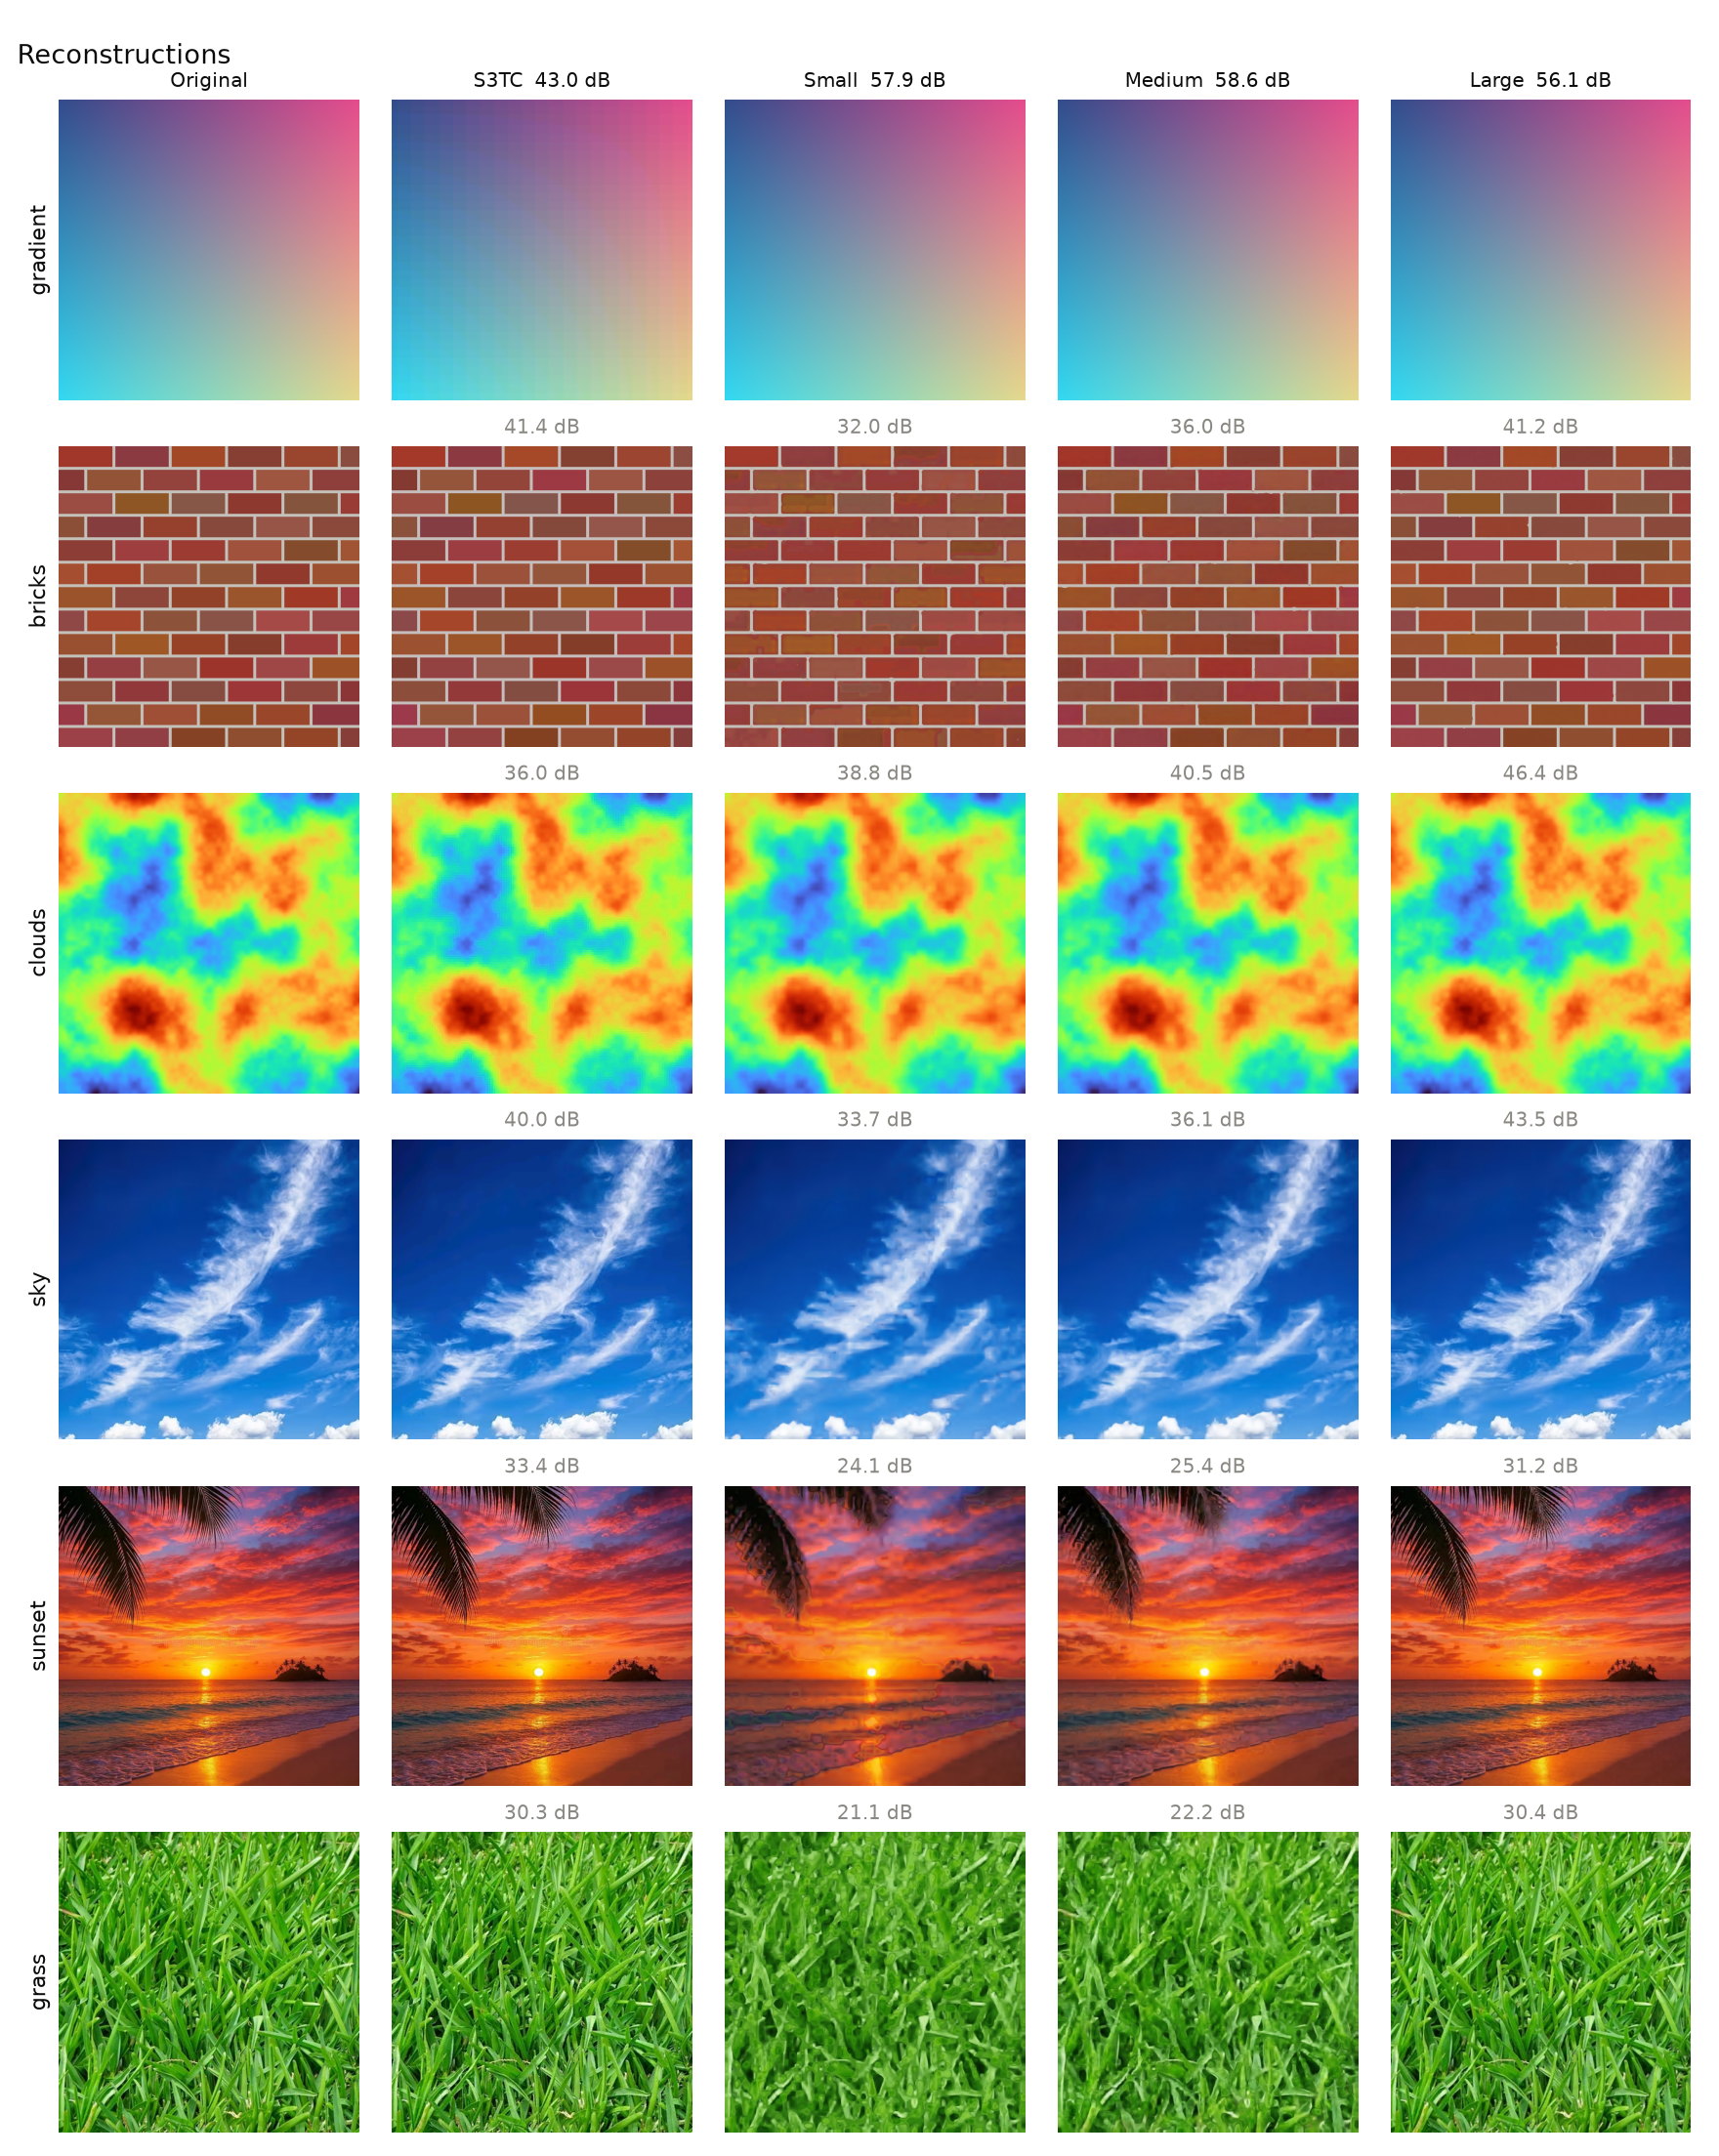
\includegraphics[width=\textwidth]{reconstructions.png}
\caption{Original, S3TC, and the three neural architectures for all six textures.}
\label{fig:recon}
\end{figure}

\begin{figure}[tbp]
\centering
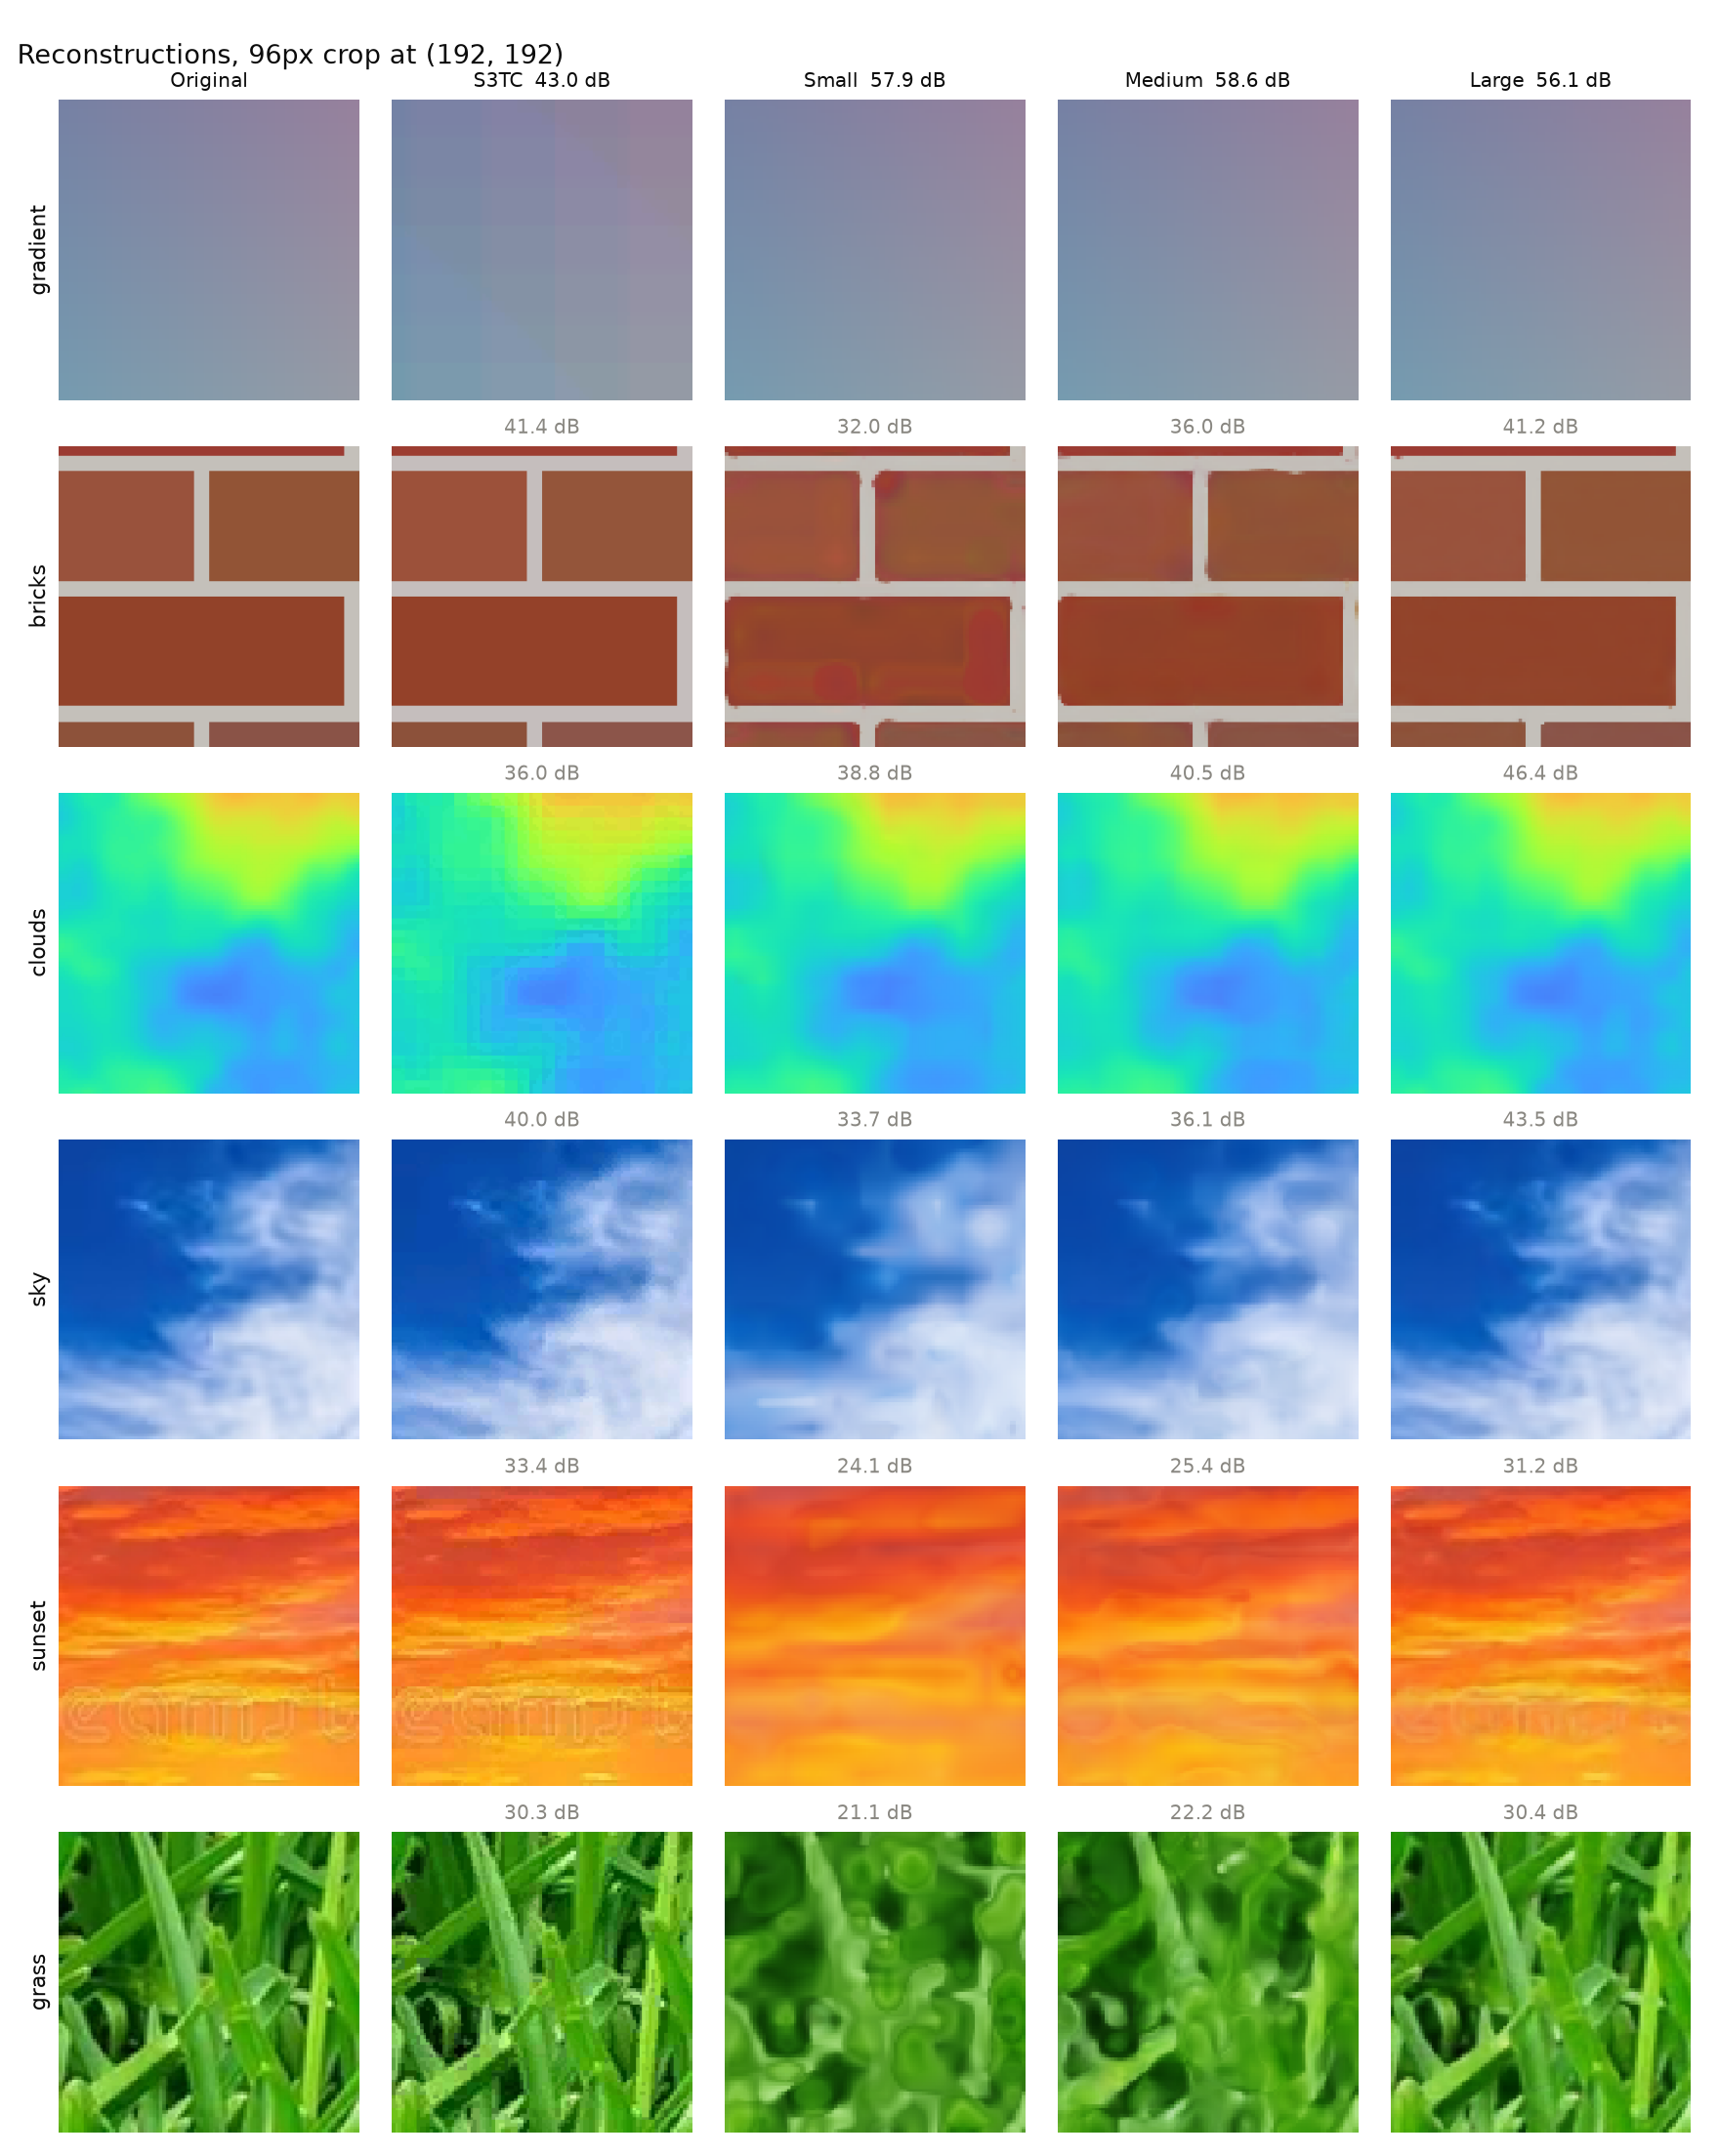
\includegraphics[width=0.92\textwidth]{crops.png}
\caption{A 96-pixel crop from each texture, enlarged with nearest-neighbor so block and cell artifacts are visible.}
\label{fig:crops}
\end{figure}

\paragraph{Where S3TC breaks down.} Look at the clouds and gradient rows of Figure~\ref{fig:crops}. Each block reproduces only four colors, and those four lie on a single line segment in RGB space between the two endpoints. A smooth ramp crossing a block is snapped to four steps, and adjacent blocks choose different endpoints, so the result is visible $4\times4$ banding on anything low-frequency. Clouds is the worst case at $36\dB$ despite having almost no fine detail, because every block is a shallow gradient. Bricks, by contrast, is mostly two-tone (brick or mortar) within each block, which a two-endpoint palette represents almost exactly, so S3TC reaches $41\dB$ there. The failure mode is not sharpness but \emph{color diversity along one axis}: any block whose colors do not lie near a line in RGB space, or that needs more than four levels along that line, loses.

\paragraph{Why green gets the extra bit.} Sixteen bits do not split evenly three ways, so one channel gets six. Green is the right one because the eye's luminance response is dominated by green (roughly $0.2R + 0.7G + 0.07B$), so quantization error in green is the most visible as a brightness error. Giving green 64 levels instead of 32 halves the most perceptible step.

\paragraph{Why $q/\text{levels}$ is not exactly what hardware does.} Hardware expands a 5-bit code to 8 bits by bit replication, $(q \ll 3) \,|\, (q \gg 2)$, and a 6-bit code by $(q \ll 2)\,|\,(q \gg 4)$. That is an integer approximation of $q \cdot 255/31$ that needs no divider. Both maps send 0 to 0 and the maximum code to 255, and in between they differ by less than one 8-bit step, so $q/\text{levels}$ is within about $0.4\%$ of full scale of the hardware value everywhere. The assignment permits the simpler form and I use it.

\section*{P6. Results and comparison}

\begin{figure}[tbp]
\centering
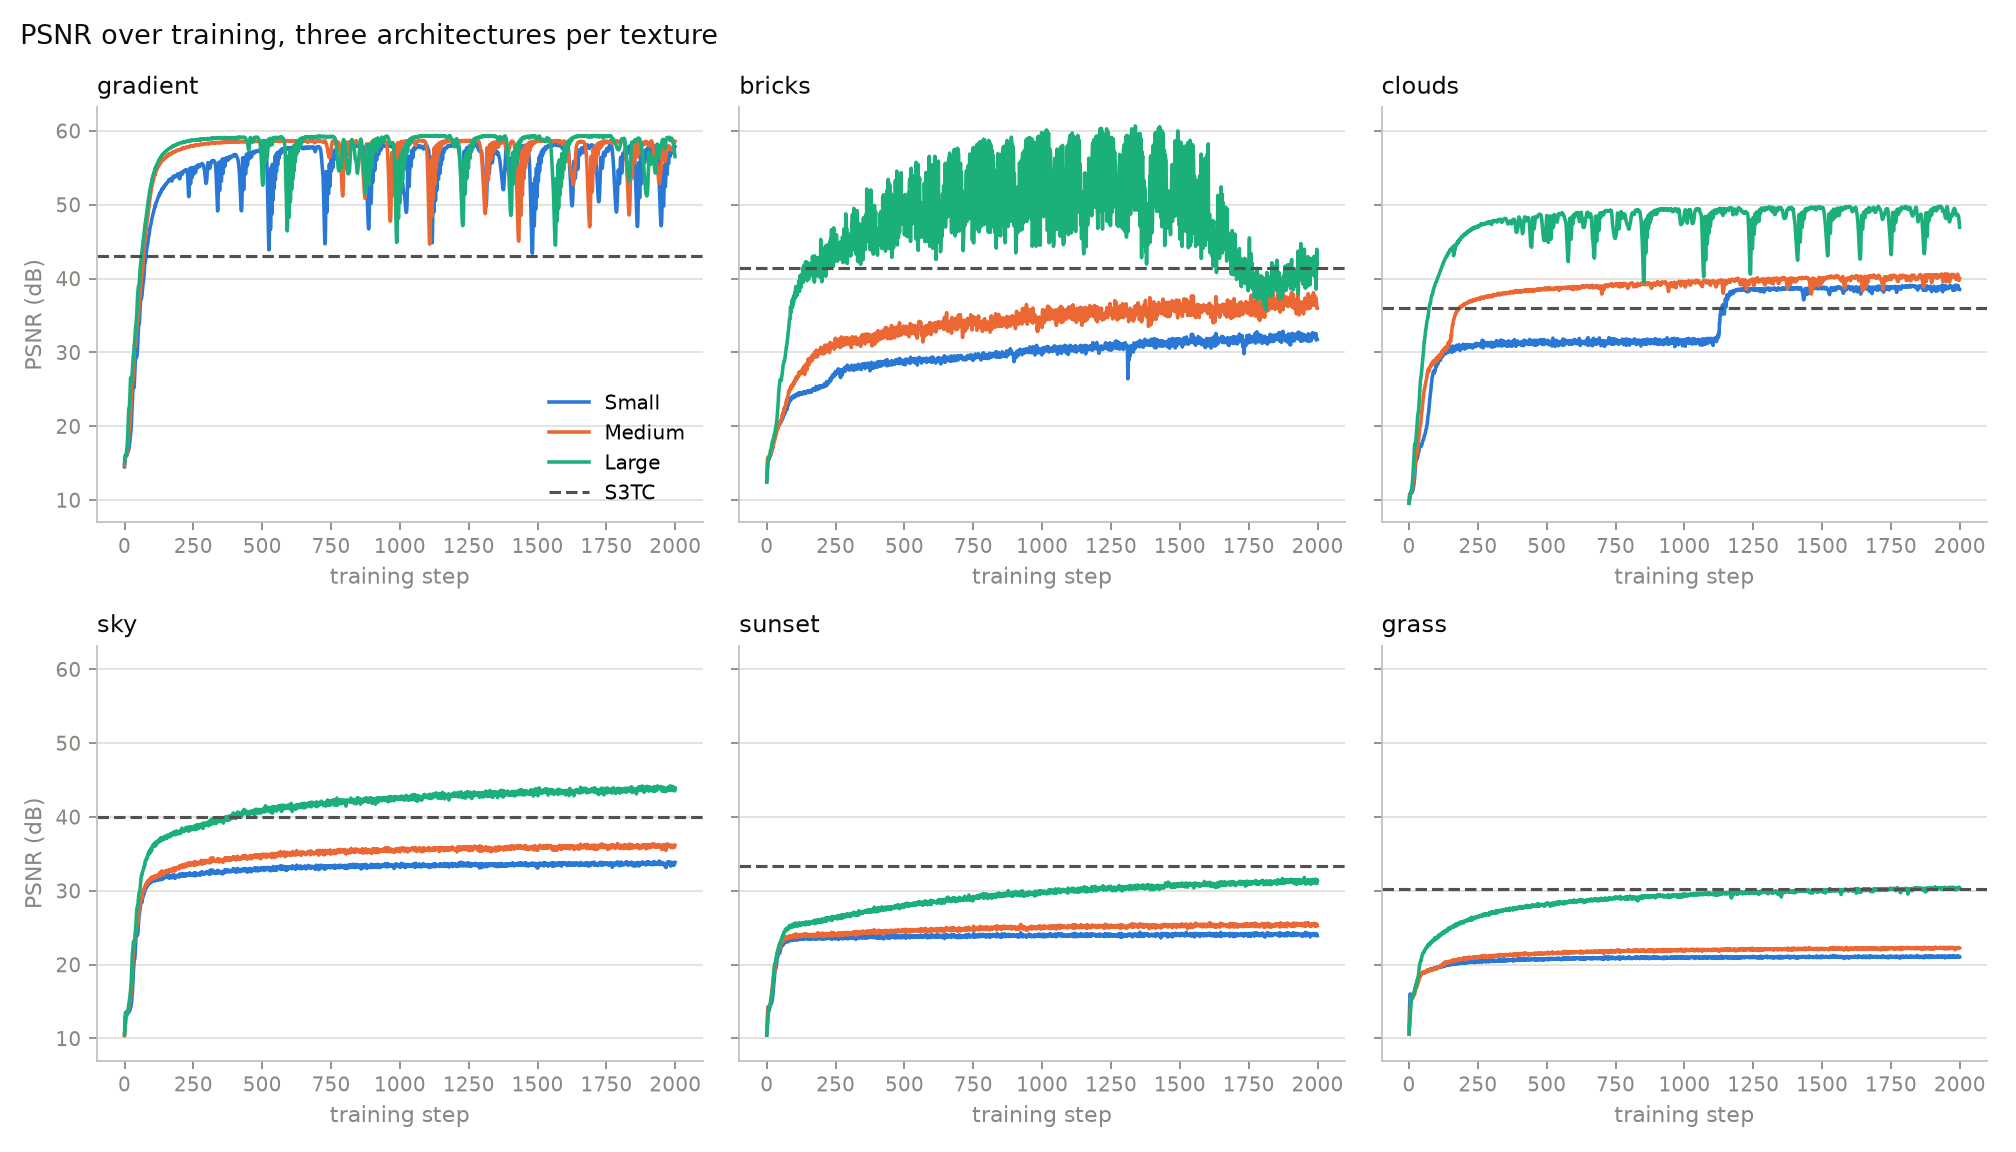
\includegraphics[width=\textwidth]{psnr_curves.png}
\caption{Minibatch PSNR over training for all architectures on all textures. Dashed line: S3TC.}
\label{fig:curves}
\end{figure}

\begin{figure}[tbp]
\centering
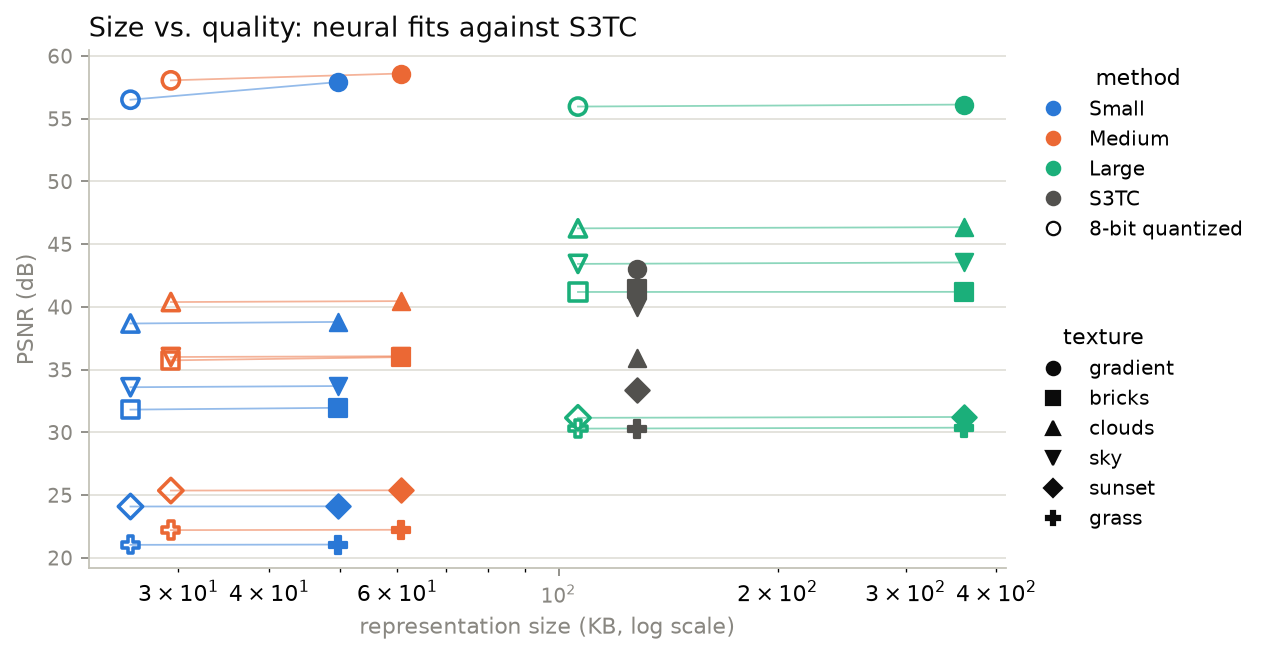
\includegraphics[width=0.8\textwidth]{size_vs_quality.png}
\caption{Size vs.\ quality. Filled markers are float32 models, hollow markers their 8-bit quantized versions (P7), gray is S3TC.}
\label{fig:size}
\end{figure}

\begin{table}[H]
\centering
\small
\begin{tabular}{llrlrrcc}
\toprule
texture & arch & PSNR & params (grid + MLP) & KB & ratio & $<$ S3TC size & $\geq$ S3TC PSNR \\
\midrule
gradient & S3TC   & 43.03 & & 128.0 & 0.1667 & & \\
gradient & Small  & 57.92 & 8,192 + 4,547 & 49.8 & 0.0648 & yes & yes \\
gradient & Medium & \textbf{58.61} & 10,752 + 4,803 & 60.8 & 0.0791 & yes & yes \\
gradient & Large  & 56.13 & 87,040 + 5,443 & 361.3 & 0.4704 & no & yes \\
\midrule
bricks & S3TC   & \textbf{41.39} & & 128.0 & 0.1667 & & \\
bricks & Small  & 31.96 & 8,192 + 4,547 & 49.8 & 0.0648 & yes & no \\
bricks & Medium & 36.00 & 10,752 + 4,803 & 60.8 & 0.0791 & yes & no \\
bricks & Large  & 41.20 & 87,040 + 5,443 & 361.3 & 0.4704 & no & tie \\
\midrule
clouds & S3TC   & 35.95 & & 128.0 & 0.1667 & & \\
clouds & Small  & 38.81 & 8,192 + 4,547 & 49.8 & 0.0648 & yes & yes \\
clouds & Medium & 40.47 & 10,752 + 4,803 & 60.8 & 0.0791 & yes & yes \\
clouds & Large  & \textbf{46.36} & 87,040 + 5,443 & 361.3 & 0.4704 & no & yes \\
\bottomrule
\end{tabular}
\caption{Nine float32 fits against S3TC (128.0~KB, ratio 0.1667). Bold marks the best PSNR per texture.}
\end{table}

\paragraph{Gradient: Medium is best,} though Small and Large are within $2.5\dB$ and all three are far past S3TC. The texture is one low-frequency ramp. The MLP plus bilinear blending already produces smooth output, so a 64-cell grid with two features has more than enough capacity, and the 128 level in Large buys nothing. Large's slightly lower number is training noise (see below), not a capacity effect. Every architecture beats S3TC on quality, and Small and Medium beat it on size at the same time. This is the content S3TC handles worst and the neural representation handles best.

\paragraph{Bricks: Large is best,} and it only ties S3TC. Bricks has sharp mortar edges every few texels. The Small grid has 64 cells across 512 texels, 8 texels per cell, so it cannot place an edge more precisely than the bilinear blend between two cells allows; Figure~\ref{fig:crops} shows the mortar smeared into soft blobs. Medium adds coarser levels but its finest level is still 64, so edges stay soft ($36\dB$). Only the 128 level in Large (4 texels per cell) resolves them, at $41\dB$. The Small-vs-Medium comparison isolates what multi-resolution buys: $4\dB$, from the coarse levels absorbing the low-frequency brick color so the 64 level can spend its capacity on edges. But fine structure still needs the fine level. S3TC is near-perfect on two-tone blocks. Small and Medium beat S3TC on size but not quality; Large matches quality at three times the size.

\paragraph{Clouds: Large is best} by a wide margin, and every architecture beats S3TC on both axes. Clouds has smooth detail at every scale, which is exactly what a multi-resolution grid represents: each level captures the octave of detail matching its cell size. It is also exactly what S3TC cannot represent, since every block is a gradient. Small alone beats S3TC by $3\dB$ at 40\% of the size.

\paragraph{Compression ratio vs.\ S3TC.} Small ($0.065$) and Medium ($0.079$) are smaller than S3TC ($0.167$) on every texture. Large in float32 ($0.470$) is nearly three times larger than S3TC; it becomes competitive only after quantization (P7). Reading Figure~\ref{fig:size} both ways: at S3TC's size (128~KB) the nearest neural point is quantized Large at 106~KB, which is better on gradient, clouds, and sky and worse on sunset; at S3TC's PSNR, Small or Medium reach it at less than half the size on gradient and clouds but never reach it on bricks, sunset, or grass.

\paragraph{A note on training stability.} Figure~\ref{fig:curves} shows that Adam at $10^{-2}$ is aggressive for these grids. Gradient exhibits periodic spikes after step 500 as the optimizer overshoots a near-perfect fit, and Large on bricks climbs to about $50\dB$ around step 1000 and then collapses to $41\dB$ by step 2000. The assignment fixes the optimizer settings so I did not change them, but the reported bricks-Large number is unlucky relative to where the run sat mid-training. A learning-rate decay would make the final number representative and is the first thing I would change in practice. Runs also vary by 1--3~dB between seeds on MPS. All numbers here are from a single run.

\section*{P7. Quantization}
\label{sec:quant}

After training, each grid level is quantized separately with its own $(\text{lo}, \text{scale})$: $q = \mathrm{round}((x - \text{lo})/\text{scale})$ stored as uint8, decoded as $\hat{x} = \text{lo} + q\cdot\text{scale}$ with $\text{scale} = (\text{hi}-\text{lo})/255$. The MLP stays float32. Size is one byte per grid value, plus 8 bytes per level for $(\text{lo},\text{scale})$, plus 4 bytes per MLP parameter.

\begin{table}[H]
\centering
\small
\begin{tabular}{llrrrrrrr}
\toprule
texture & arch & PSNR f32 & PSNR 8-bit & loss & KB f32 & KB 8-bit & ratio 8-bit & factor \\
\midrule
gradient & Small  & 57.92 & 56.52 & 1.40 & 49.8 & 25.8 & 0.0336 & 29.8$\times$ \\
gradient & Medium & 58.61 & 58.06 & 0.55 & 60.8 & 29.3 & 0.0381 & 26.2$\times$ \\
gradient & Large  & 56.13 & 55.97 & 0.16 & 361.3 & 106.3 & 0.1384 & 7.2$\times$ \\
bricks & Small  & 31.96 & 31.82 & 0.14 & 49.8 & 25.8 & 0.0336 & 29.8$\times$ \\
bricks & Medium & 36.00 & 35.74 & 0.26 & 60.8 & 29.3 & 0.0381 & 26.2$\times$ \\
bricks & Large  & 41.20 & 41.19 & 0.01 & 361.3 & 106.3 & 0.1384 & 7.2$\times$ \\
clouds & Small  & 38.81 & 38.68 & 0.13 & 49.8 & 25.8 & 0.0336 & 29.8$\times$ \\
clouds & Medium & 40.47 & 40.39 & 0.08 & 60.8 & 29.3 & 0.0381 & 26.2$\times$ \\
clouds & Large  & 46.36 & 46.26 & 0.10 & 361.3 & 106.3 & 0.1384 & 7.2$\times$ \\
\bottomrule
\end{tabular}
\caption{PSNR and size before and after 8-bit quantization of the grids.}
\end{table}

The hollow markers in Figure~\ref{fig:size} show each quantized model joined to its float32 twin: the points slide left by 2--3.4$\times$ with almost no vertical movement.

\paragraph{How much quality was lost and why.} Under $0.3\dB$ in eight of nine cases. Each grid level's values span a range of a few units, so 256 buckets give a step of roughly $0.01$--$0.03$, and the rounding error that introduces is far below the model's own reconstruction error, which is what dominates PSNR. The exception is gradient-Small at $1.4\dB$: that model was already so close to perfect ($58\dB$, MSE about $1.6\times10^{-6}$) that quantization noise became the dominant error term. Quantization costs little unless the model is already nearly exact.

\paragraph{Why size did not drop a full $4\times$.} The MLP stays float32. For Small the MLP is 18~KB of the 26~KB total and now dominates. Quantizing the MLP too (supported by the code, not reported) would bring Small to about 12~KB. For Large the grid dominates and the drop is $3.4\times$.

\paragraph{Effect on the S3TC comparison.} After quantization, Large lands at 106~KB, below S3TC's 128~KB, while matching or beating S3TC's PSNR on all three textures. Before quantization it was three times larger. Quantization is what makes the large-grid model a fair competitor.

\section*{P8. Self-sourced textures}

\begin{figure}[tbp]
\centering

\includegraphics[width=0.31\textwidth]{sky.png}\hfill
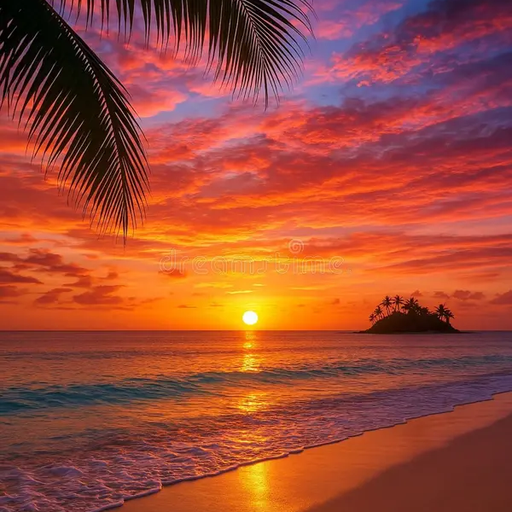
\includegraphics[width=0.31\textwidth]{sunset.png}\hfill
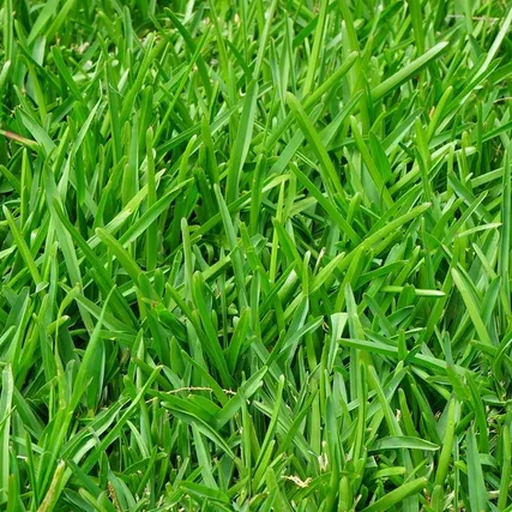
\includegraphics[width=0.31\textwidth]{grass.png}
\caption{Sky, sunset, and grass, each center-cropped and resized to $512\times512$.}
\end{figure}

Three photographs chosen to spread across the frequency axis: \textbf{sky} (smooth blue with thin cirrus wisps), \textbf{sunset} (broad color gradients broken by dark palm fronds and wave foam), and \textbf{grass} (fine blade edges everywhere). Sky and grass were upscaled slightly from about 400~px, which softens their finest detail; the sunset carries a stock-photo watermark, which adds a few sharp edges. To quantify content I measure the fraction of spectral energy above 32 cycles per image width, which is the Nyquist limit of the 64-cell grid: the share of the texture the Small model cannot resolve at all.

\begin{table}[H]
\centering
\small
\begin{tabular}{lrrrrrr}
\toprule
texture & high-freq fraction & S3TC & Small & Medium & Large & Large 8-bit \\
\midrule
gradient & 0.019 & 43.03 & 57.92 & 58.61 & 56.13 & 55.97 \\
clouds   & 0.018 & 35.95 & 38.81 & 40.47 & 46.36 & 46.26 \\
sky      & 0.025 & 40.01 & 33.70 & 36.07 & 43.54 & 43.43 \\
sunset   & 0.191 & 33.39 & 24.11 & 25.38 & 31.23 & 31.16 \\
bricks   & 0.471 & 41.39 & 31.96 & 36.00 & 41.20 & 41.19 \\
grass    & 0.513 & 30.26 & 21.06 & 22.24 & 30.38 & 30.30 \\
\bottomrule
\end{tabular}
\caption{Final PSNR (dB) for all six textures, ordered by high-frequency content. Sizes: S3TC 128~KB, Small 49.8~KB, Medium 60.8~KB, Large 361~KB, Large 8-bit 106~KB.}
\end{table}

\begin{figure}[tbp]
\centering
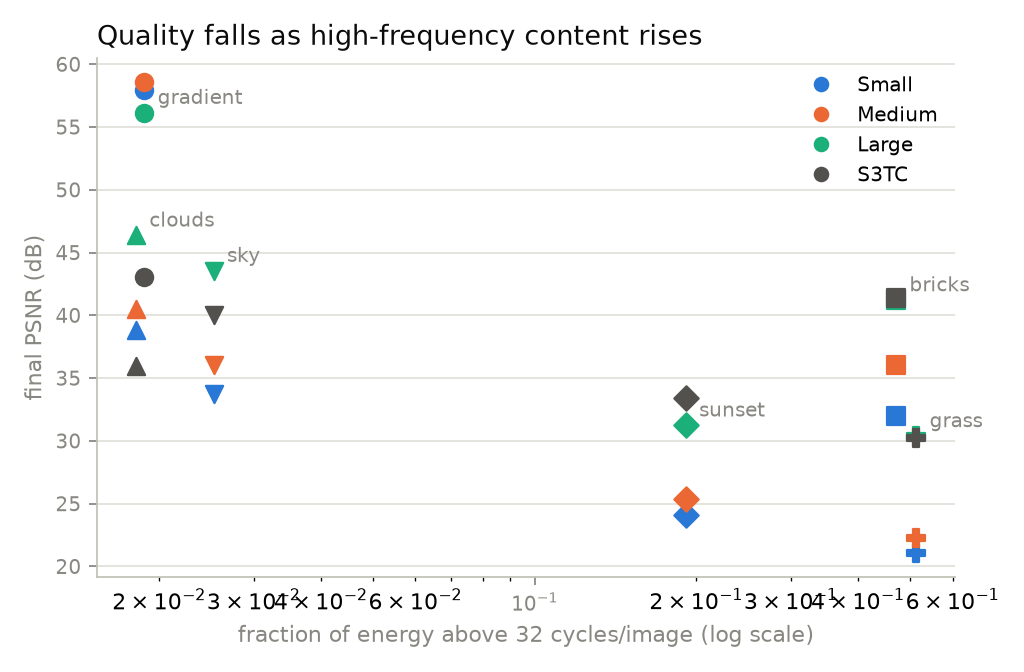
\includegraphics[width=0.8\textwidth]{psnr_vs_frequency.png}
\caption{Final PSNR against each texture's high-frequency energy fraction.}
\label{fig:freq}
\end{figure}

\paragraph{Sky} sits with the smooth textures on the frequency axis but behaves differently from clouds: only Large beats S3TC. The difference is the cirrus wisps, which are thin and bright against a dark background. They contribute little total energy, so the metric calls sky smooth, but reproducing them needs the 128 level. Small and Medium blur them and lose 4--6~dB to S3TC. S3TC does well because most blocks are blue with a little white, which is a two-endpoint palette.

\paragraph{Sunset} is the middle case and the one where S3TC wins outright, even against Large. The gradients are easy for every model, but the palm fronds are dark, thin, and high-contrast, and the wave foam is fine texture. Small paints the fronds as blobs (Figures~\ref{fig:recon} and~\ref{fig:crops}). S3TC handles dark-on-bright edges almost perfectly and its banding on the sky gradient is mild at this resolution, so it comes out $2\dB$ ahead of Large at a third of Large's float32 size.

\paragraph{Grass} is the worst case for the neural method, as designed. Half of its spectral energy sits above what even the 128 level can represent. Small and Medium are 8--9~dB below S3TC and look like green paint; Large only ties S3TC at $2.8\times$ the size in float32 ($0.83\times$ after quantization). Content that is high-frequency everywhere gives a feature grid nothing to exploit: there is no coarse structure for the coarse levels to absorb, and the fine level is not fine enough.

\paragraph{The overall picture.} Across all six textures, final PSNR falls with the high-frequency fraction almost monotonically for every architecture, and the gap between Small and Large grows with it, from about zero on gradient to $9\dB$ on grass. That gap is exactly what the fine grid level buys. The neural representation wins decisively on smooth, multi-scale content (gradient, clouds), where S3TC's four-colors-per-block limit shows as banding. S3TC wins on content that is locally two-tone with hard edges (bricks, sunset fronds) and on content finer than the grid (grass). After 8-bit quantization the Large model is smaller than S3TC on every texture and matches or beats its quality on five of six, losing only on sunset.

\end{document}
